% Provenance (never printed): the long-run growth strand of ../economics_series.md
% (facts before models; Maddison's long series). Brief: sources/book1/BRIEFS.md, g6-02.
% Chart data: figdata/grade-6/02-living-standards (Maddison 2023; Nordhaus 1996, Table 1.6).
\chapter{Two Hundred Years of Living Standards}\label{ch:g6:living-standards}

In 1700, a family in England had about twice the \omterm{def:g6:living-standards:income-per-person}{income per person} of a family
four hundred years earlier: a slow rise, measured in centuries. It ate mostly bread, lit its house with a
fire or a few candles, and walked wherever it went. In 2022, a family in the
same country earned about sixteen times as much per person as in 1700. This
chapter follows that change, which began in a few countries around 1800 and
has spread, unevenly, to most of the world.

\begin{recall}
A \omterm{def:g6:reading-economic-charts:per-person}{per-person value} is a total divided by the number of people
(\cref{def:g6:reading-economic-charts:per-person}). On a \omterm{def:g6:reading-economic-charts:times-ten-scale}{times-ten scale}, each
gridline is ten times the one below it, and equal distances mean ``the same
number of times larger'' (\cref{def:g6:reading-economic-charts:times-ten-scale}).
\end{recall}

\section{Income per person, and what it measures}

To compare how well people live in different years and places, economists
start with one number.

\begin{definition}[Income per person]\label{def:g6:living-standards:income-per-person}
The \emph{income per person}\index{income per person} of a country in a year
is the value of everything its people produce in that year, divided by the
number of people. It is measured in dollars of \emph{fixed purchasing power}:
dollars that buy the same amount of goods in every year and every country.
\end{definition}

The charts of this chapter use ``2011 dollars'': each dollar buys what a
dollar bought in the United States in 2011. So when \omterm{def:g6:living-standards:income-per-person}{income per person} goes
from 3\,000 to 30\,000 of these dollars, people can really buy ten times as
much, not merely pay higher prices. How such dollars are built is explained in
grade~9.

\begin{definition}[Living standard]\label{def:g6:living-standards:living-standard}
The \emph{living standard}\index{living standard} of a group of people is
how well they live: what they can eat, wear and use, the house they live in,
their health, how long they live and how much they learn. \omterm{def:g6:living-standards:income-per-person}{Income per person}
measures only one part of it, the part that money can buy.
\end{definition}

\omterm{def:g6:living-standards:income-per-person}{Income per person} is the most used measure of \omterm{def:g6:living-standards:living-standard}{living standards} because it can
be estimated for almost every country and for many centuries. The next
chapters add the other parts: poverty, health, school and work.

\begin{measure}[Income per person over centuries]
Nobody counted the income of England in 1300. Researchers rebuild it from
what survives: the wages written in the account books of farms, colleges and
building sites; the prices of wheat, beer and cloth in market records; the
harvests of manors; and tax lists that count people. From wages and prices
they estimate what a worker could buy; from harvests and trades they estimate
how much was produced. Each estimate could be wrong by a fifth or more. The
Maddison Project Database collects the estimates of many such studies, country
by country, and turns them into 2011 dollars, so that they can be drawn on one
chart. Before 1820, it has estimates for only a few countries.
\end{measure}

\section{Centuries of almost nothing, then a take-off}

\begin{omchart}{Income per person, 1300--2022, in 2011 dollars, on a times-ten
scale: the United Kingdom (England before 1700), the Netherlands, and the
whole world (the source's world estimate, from 1820).}{Maddison Project Database 2023: GDP per person (United Kingdom, Netherlands) and regional data (world)}
\begin{tikzpicture}
\begin{semilogyaxis}[omtimesten, xmin=1300, xmax=2022, ymin=500, ymax=100000,
  xtick={1300,1400,1500,1600,1700,1800,1900,2000}, xlabel={Year},
  ylabel={Dollars per person}, legend pos=north west]
\addplot table[x=year, y=gbr]
  {figdata/grade-6/02-living-standards/out/long_run_income.csv};
\addplot table[x=year, y=nld]
  {figdata/grade-6/02-living-standards/out/long_run_income.csv};
\addplot+[mark=*, mark size=1.2pt] table[x=year, y=world]
  {figdata/grade-6/02-living-standards/out/long_run_income.csv};
\legend{United Kingdom, Netherlands, World}
\end{semilogyaxis}
\end{tikzpicture}
\end{omchart}

% figdata: long_run_income (gbr 1300 1159, 1700 2412, 1800 3343, 2022 38406; nld 1600 4270,
% 1800 4184; first year above 3000 for gbr: 1761)
For five hundred years, the line of the United Kingdom stays low. \omterm{def:g6:living-standards:income-per-person}{Income per
person} was $1\,159$ dollars in 1300 and $2\,412$ dollars in 1700: it took four
centuries to double. It first passed $3\,000$ dollars in the 1760s. Then the
line turns upward and never comes back: $3\,343$ dollars in 1800, $38\,406$ in
2022. The Netherlands became rich early, in the 1500s and 1600s, through trade
and shipping: $4\,270$ dollars in 1600. But two hundred years later, in 1800,
it was still at $4\,184$ dollars. A country could become richer for a while
and then stop. What happened after 1800 was different: the rise went on, year
after year, for two centuries.

\begin{definition}[Take-off]\label{def:g6:living-standards:take-off}
A country's \emph{take-off}\index{take-off (of growth)} is the moment when
its \omterm{def:g6:living-standards:income-per-person}{income per person} starts to rise and keeps rising for many decades, instead
of rising for a while and then falling back.
\end{definition}

\begin{omfigure}
\begin{tikzpicture}[econ, x=1cm, y=1cm]
  % widths: years / 100 x 2 cm; heights: multiplication factor x 0.35 cm.
  % figdata: long_run_income (gbr 1300 1159, 1800 3343 -> x2.9; 1820 3306, 2022 38406 -> x11.6)
  \fill[omDef!25] (0,0) rectangle (10,{2.9*0.35});
  \draw[omDef] (0,0) rectangle (10,{2.9*0.35});
  \fill[omThm!35] (10.4,0) rectangle ({10.4+2*2.02},{11.6*0.35});
  \draw[omThm] (10.4,0) rectangle ({10.4+2*2.02},{11.6*0.35});
  \node[font=\footnotesize, align=center] at (5,1.65) {1300 to 1800: 500 years\\income per person $\times 2.9$};
  \node[font=\footnotesize, align=center, fill=white, inner sep=1pt] at ({10.4+2.02},{11.6*0.35/2}) {1820 to 2022:\\202 years\\$\times 11.6$};
  \node[below, font=\scriptsize] at (0,0) {1300};
  \node[below left, font=\scriptsize, inner xsep=0pt] at (10,0) {1800};
  \node[below right, font=\scriptsize, inner xsep=0pt] at (10.4,0) {1820};
  \node[below, font=\scriptsize] at ({10.4+4.04},0) {2022};
\end{tikzpicture}

{\small \omterm{def:g6:living-standards:income-per-person}{Income per person} in the United Kingdom: the width of each block is the
number of years, its height is how many times \omterm{def:g6:living-standards:income-per-person}{income per person} was multiplied.
The narrow, tall block on the right is the \omterm{def:g6:living-standards:take-off}{take-off}.}
\end{omfigure}

The \omterm{def:g6:living-standards:take-off}{take-off} is the largest change in how people live since farming began. It
came with new machines driven by coal and steam, new ways of organising work,
more trade, and more people who could read. Which of these mattered most, and
why it started in north-western Europe, is still studied; later books of this
course present the models economists use to explain growth.

\section{First, later, not yet: the regions since 1820}

The \omterm{def:g6:living-standards:take-off}{take-off} did not reach the whole world at once. The next chart draws
\omterm{def:g6:living-standards:income-per-person}{income per person} for five of the eight large regions used by the source.

\begin{omchart}{Income per person in five regions, 1820--2022, in 2011 dollars, on
a times-ten scale. The dots are the years for which the source gives a regional
estimate. ``Western Offshoots'' are the United States, Canada, Australia and New
Zealand.}{Maddison Project Database 2023, regional data: GDP per person}
\begin{tikzpicture}
\begin{semilogyaxis}[omtimesten, xmin=1820, xmax=2022, ymin=500, ymax=100000,
  xtick={1820,1860,1900,1940,1980,2020}, xlabel={Year},
  ylabel={Dollars per person}, legend pos=north west,
  every axis plot/.append style={mark=*, mark size=0.9pt}]
\addplot table[x=year, y=western_offshoots]
  {figdata/grade-6/02-living-standards/out/income_by_region.csv};
\addplot table[x=year, y=western_europe]
  {figdata/grade-6/02-living-standards/out/income_by_region.csv};
\addplot table[x=year, y=latin_america]
  {figdata/grade-6/02-living-standards/out/income_by_region.csv};
\addplot table[x=year, y=east_asia]
  {figdata/grade-6/02-living-standards/out/income_by_region.csv};
\addplot table[x=year, y=ssa]
  {figdata/grade-6/02-living-standards/out/income_by_region.csv};
\legend{Western Offshoots, Western Europe, Latin America, East Asia, Sub-Saharan Africa}
\end{semilogyaxis}
\end{tikzpicture}
\end{omchart}

% figdata: income_by_region (1820: wo 2513, we 2171, la 957, ea 911, ssa 1188;
% 1950: ea 1109, ssa 1327; 2022: wo 56568, we 41323, la 14028, ea 21729, ssa 3437)
In 1820, all five regions were poor, and close together: the richest, the
Western Offshoots, had $2\,513$ dollars per person, less than three times East
Asia's $911$. Then the regions split apart, in three groups.

\begin{itemize}
  \item \textbf{First}: Western Europe and the Western Offshoots took off in the
        1800s and rose steadily. In 2022 they had $41\,323$ and $56\,568$ dollars
        per person.
  \item \textbf{Later}: East Asia barely moved for 130 years ($1\,109$ dollars
        in 1950), then rose faster than any region had ever risen, to $21\,729$
        dollars in 2022. Latin America rose earlier but more slowly, with long
        pauses.
  \item \textbf{Not yet}: Sub-Saharan Africa rose from $1\,327$ dollars in 1950 to
        $3\,437$ in 2022. It is still the poorest region of the chart.
\end{itemize}

In 1820, the richest region of the chart had less than three times the income of
the poorest. In 2022, it had more than sixteen times as much ($56\,568 \div
3\,437 \approx 16.5$). The \omterm{def:g6:living-standards:take-off}{take-off} made most of the world richer, and it also
made the gaps between regions much wider.

\section{Catching up since 1950: six paths}

A country that starts poor can grow faster than the rich countries for a
while, and close part of the gap.

\begin{definition}[Catch-up]\label{def:g6:living-standards:catch-up}
A poorer country \emph{catches up}\index{catch-up} with a richer one when its
\omterm{def:g6:living-standards:income-per-person}{income per person} grows faster, so that the ratio between the richer country's
\omterm{def:g6:living-standards:income-per-person}{income per person} and its own gets smaller.
\end{definition}

Catching up is possible, but it is not automatic. The next chart follows six
countries since 1950: three that caught up a great deal, and three that did not.

\begin{omchart}{Income per person in six countries, 1950--2022, in 2011 dollars,
on a times-ten scale.}{Maddison Project Database 2023: GDP per person}
\begin{tikzpicture}
\begin{semilogyaxis}[omtimesten, xmin=1950, xmax=2022, ymin=100, ymax=100000,
  xtick={1950,1960,1970,1980,1990,2000,2010,2020}, xlabel={Year},
  ylabel={Dollars per person}, height=0.62\linewidth,
  legend style={at={(0.5,-0.2)}, anchor=north, legend columns=3},
  cycle list={{omDef, thick}, {omThm, thick}, {omMeth, thick},
    {omDef, thick, densely dashed}, {omThm, thick, densely dashed},
    {omMeth, thick, densely dashed}}]
\addplot table[x=year, y=kor] {figdata/grade-6/02-living-standards/out/six_paths.csv};
\addplot table[x=year, y=chn] {figdata/grade-6/02-living-standards/out/six_paths.csv};
\addplot table[x=year, y=bwa] {figdata/grade-6/02-living-standards/out/six_paths.csv};
\addplot table[x=year, y=arg] {figdata/grade-6/02-living-standards/out/six_paths.csv};
\addplot table[x=year, y=ven] {figdata/grade-6/02-living-standards/out/six_paths.csv};
\addplot table[x=year, y=cod] {figdata/grade-6/02-living-standards/out/six_paths.csv};
\legend{South Korea, China, Botswana, Argentina, Venezuela, DR Congo}
\end{semilogyaxis}
\end{tikzpicture}
\end{omchart}

% figdata: six_paths (1950: kor 998, chn 799, bwa 489, arg 7949, ven 8462, cod 909;
% 2022: kor 41321, chn 19238, bwa 16352, arg 18292, ven 5267, cod 844; ven 2012 18486;
% kor first above arg 1988; chn first above arg 2020)
The solid lines climb steeply. In 1950, South Korea had $998$ dollars per
person, China $799$ and Botswana $489$: they were among the poorest countries in
the world. In 2022, South Korea had $41\,321$ dollars, more than forty times its
1950 income; China had $19\,238$ and Botswana $16\,352$.

The dashed lines tell other stories. Argentina and Venezuela were far richer
than South Korea in 1950 ($7\,949$ and $8\,462$ dollars). Argentina grew slowly,
with deep falls, to $18\,292$ dollars in 2022; South Korea passed it in 1988,
and China in 2020. Venezuela rose until 2012 ($18\,486$ dollars) and then
collapsed, to $5\,267$ dollars in 2022, less than in 1950. The Democratic
Republic of the Congo had $909$ dollars per person in 1950 and $844$ in 2022:
seventy years without a rise.

\begin{example}[The gap between South Korea and Argentina]\label{ex:g6:living-standards:gap}
In 1950, Argentina's \omterm{def:g6:living-standards:income-per-person}{income per person} was $7\,949 \div 998 \approx 8.0$ times
South Korea's. In 2022, South Korea's was $41\,321 \div 18\,292 \approx 2.3$
times Argentina's. On the times-ten chart, the two lines cross in 1988; before,
the dashed line is above, after, the solid one.
\end{example}

Why some countries caught up and others did not is one of the largest
questions of economics. The chart cannot answer it; it shows only that the
answer is not ``rich countries stay rich and poor countries stay poor''.

\section{What an hour of work buys}

Dollars of 2011 are an abstract unit. Another way to compare \omterm{def:g6:living-standards:living-standard}{living standards}
across centuries is to ask a concrete question: how long must a worker work to
buy a given thing?

\begin{omfigure}

\includegraphics[width=0.62\linewidth]{images/book1/ai/g6-living-standards-bakery.jpg}

{\small A family buys bread. How many minutes of work a loaf costs, then and
now, is one way to compare \omterm{def:g6:living-standards:living-standard}{living standards} across two centuries.}
\end{omfigure}

Light is a good example, because a candle and an electric lamp give the same
thing --- light --- and light can be measured. Physicists measure an amount of
light in \emph{lumen-hours}; 1\,000 lumen-hours is roughly the light of one
bright household bulb burning for one hour.

\begin{omchart}{The work needed to pay for 1\,000 lumen-hours of light in the
United States, 1800--1992, in hours of work at the wage of the time, on a
times-ten scale. Each dot is one kind of lamp in one year.}{Nordhaus (1996),
Table 1.6, labour price of light}
\begin{tikzpicture}
\begin{semilogyaxis}[omtimesten, xmin=1790, xmax=2030, ymin=0.0001, ymax=10,
  ytickten={-4,...,1}, xtick={1800,1850,1900,1950,2000}, xlabel={Year},
  ylabel={Hours of work}, yticklabel style={/pgf/number format/precision=4},
  nodes near coords, point meta=explicit symbolic,
  visualization depends on={value \thisrow{pos} \as \labelpos},
  every node near coord/.append style={font=\scriptsize, anchor=\labelpos,
    inner sep=4pt}]
\addplot+[mark=*, mark size=1.5pt] table[x=year, y=hours, meta=device]
  {figdata/grade-6/02-living-standards/out/light.csv};
\end{semilogyaxis}
\end{tikzpicture}
\end{omchart}

% ledger: g6:light-candle-1800, g6:light-filament-1900, g6:light-fluorescent-1992
In 1800, 1\,000 lumen-hours of candlelight cost $5.37$ hours of work: more than
five hours of work for one hour of good light. In 1900, an electric lamp gave
the same light for $0.22$ hour of work, about thirteen minutes. In 1992, a
low-energy lamp gave it for $0.000119$ hour of work: less than half a second.
On the times-ten chart, the dots fall by almost five steps, and five steps would
mean $100\,000$ times. The labour price of light was divided by about
$45\,000$ ($5.37 \div 0.000119$).

\begin{omfigure}
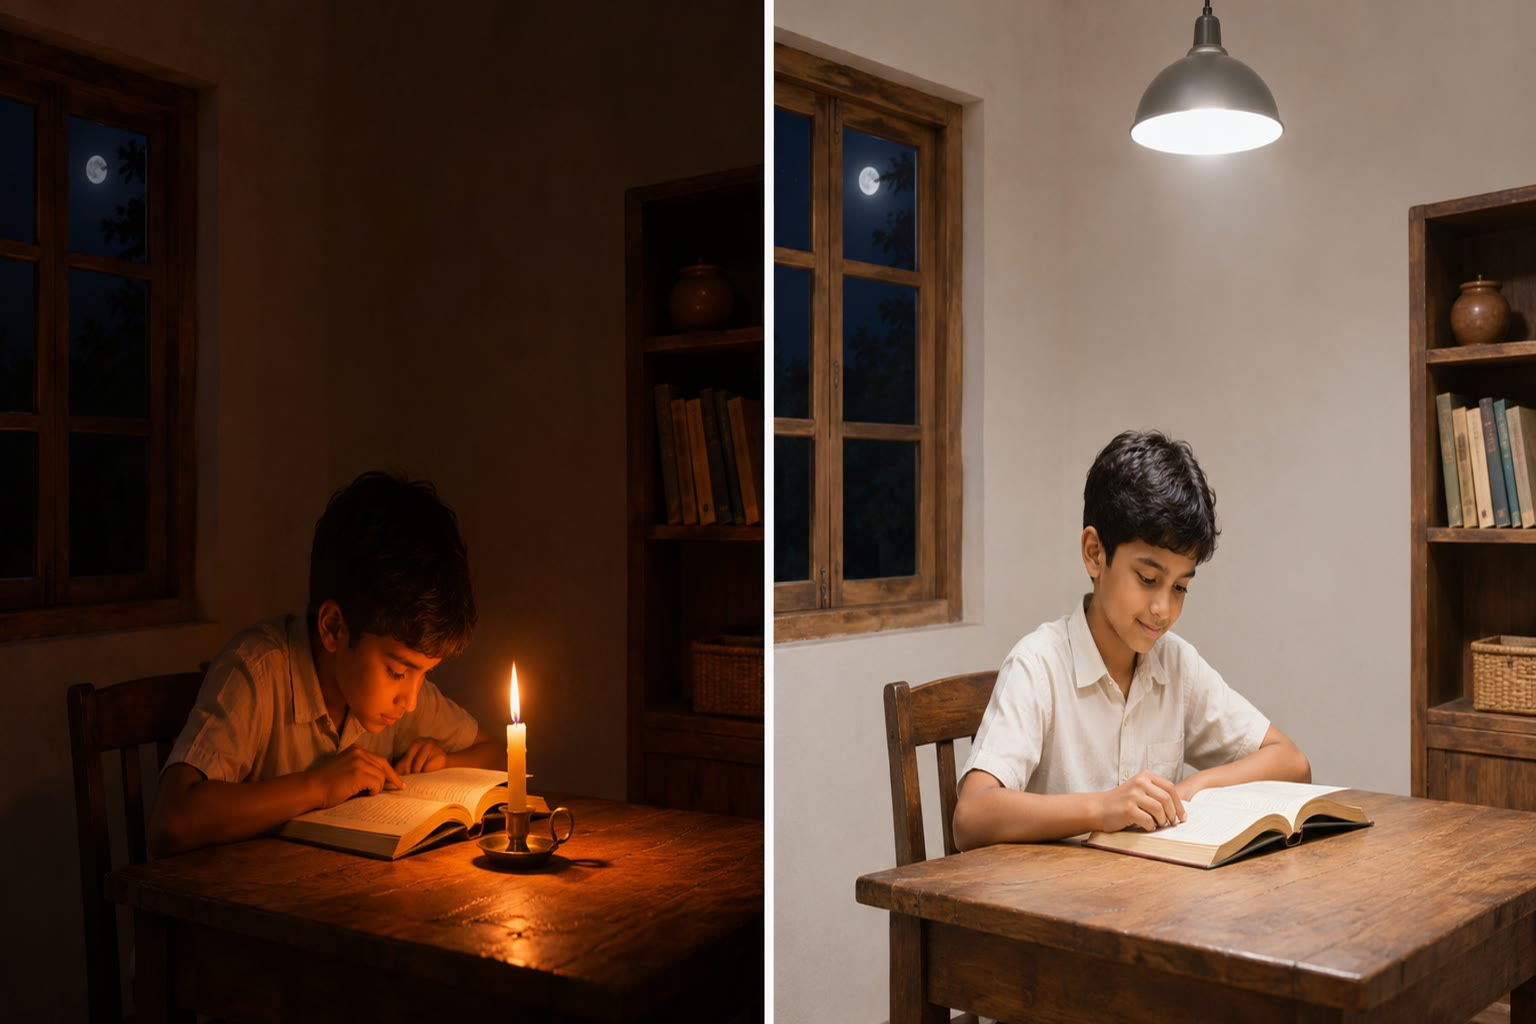
\includegraphics[width=0.62\linewidth]{images/book1/ai/g6-living-standards-light.jpg}

{\small The same room lit by a candle and by an electric lamp. Two centuries ago,
most families went to bed when it got dark, because light was dear.}
\end{omfigure}

\begin{measure}[What an hour of work buys]
To measure the ``labour price'' of something, divide its price by the wage
for one hour of work, both in the money of the same year:
\[
  \text{hours of work} = \frac{\text{price}}{\text{wage per hour}}.
\]
The money units cancel, so no correction for prices is needed. For light,
Nordhaus (1996) collected the prices of candles, oil, gas
and electricity, measured how much light each kind of lamp gives, and
divided by the wages of ordinary workers in the United States. He found that
the usual price statistics, which do not count how much better new lamps are,
miss most of the fall in the price of light.
\end{measure}

\section{What an average hides}

\omterm{def:g6:living-standards:income-per-person}{Income per person} is an average. It says what each person would get if the
whole income were shared out equally, and it never is. Two countries with the
same \omterm{def:g6:living-standards:income-per-person}{income per person} can be very different places to live.

\begin{example}[Two towns with the same average]\label{ex:g6:living-standards:towns}
Two invented towns each have 1\,000 people and an income of 20\,000 dalens per
person. In the first town, every family has between 15\,000 and 25\,000 dalens
per person. In the second, 100 people have 110\,000 dalens each, and the other
900 people have 10\,000 dalens each:
\[
  \frac{100 \times 110\,000 + 900 \times 10\,000}{1\,000}
  = \frac{11\,000\,000 + 9\,000\,000}{1\,000} = 20\,000.
\]
The averages are equal. But in the second town, nine people in ten live on half
the average.
\end{example}

An average also hides what money cannot buy, and what is not sold. A rise in
\omterm{def:g6:living-standards:income-per-person}{income per person} does not say whether people are healthier, safer or freer;
it does not count the work done at home, the cleaner or dirtier air, or the
hours of rest. So economists look at several measures together. The next
chapter counts the people who are poor; the chapter after it, how long people
live.

\section{Exercises}

\begin{exercise}[$\star$]\label{exo:g6:living-standards:1}
Use the chart of \omterm{def:g6:living-standards:income-per-person}{income per person} from 1300. About how much was \omterm{def:g6:living-standards:income-per-person}{income per
person} in the United Kingdom in 1700, and in 2000? Give round numbers.
\end{exercise}

\begin{exercise}[$\star$]\label{exo:g6:living-standards:2}
Use the chart of the five regions. (a) Which region was the richest in 1820?
(b) Which was the richest in 2022, and which the poorest?
\end{exercise}

\begin{exercise}[$\star$]\label{exo:g6:living-standards:3}
% figdata: long_run_income (world 1820 1128, 2022 16677)
The world's \omterm{def:g6:living-standards:income-per-person}{income per person} was $1\,128$ dollars in 1820 and $16\,677$ dollars
in 2022. How many times larger was it in 2022? Round to one decimal.
\end{exercise}

\begin{exercise}[$\star$]\label{exo:g6:living-standards:4}
Use the chart of the six paths. (a) In 1950, which was richer, South Korea or
Argentina? (b) In about which year did the line of South Korea cross the line
of Argentina?
\end{exercise}

\begin{exercise}[$\star\star$]\label{exo:g6:living-standards:5}
% figdata: six_paths (bwa 1950 489, 2022 16352)
Botswana's \omterm{def:g6:living-standards:income-per-person}{income per person} was $489$ dollars in 1950 and $16\,352$ dollars in
2022. (a) Compute the \omterm{def:g6:reading-economic-charts:rate-of-change}{rate of change} between the two years. (b) How many times
larger was it in 2022?
\end{exercise}

\begin{exercise}[$\star\star$]\label{exo:g6:living-standards:6}
% ledger: g6:light-candle-1800, g6:light-filament-1900
1\,000 lumen-hours of light cost $5.37$ hours of work with candles in 1800, and
$0.22$ hour of work with an electric lamp in 1900. (a) How many minutes of work
is $0.22$ hour? (b) How many times less work did the same light cost in 1900
than in 1800? Round to a whole number.
\end{exercise}

\begin{exercise}[$\star\star$]\label{exo:g6:living-standards:7}
% figdata: six_paths (2022: kor 41321, cod 844)
In 2022, \omterm{def:g6:living-standards:income-per-person}{income per person} was $41\,321$ dollars in South Korea and $844$ dollars
in the Democratic Republic of the Congo. (a) How many times richer, per person,
was South Korea? Round to a whole number. (b) On the six-paths chart, are the two
lines more or less than one gridline apart? More or less than two?
\end{exercise}

\begin{exercise}[$\star\star$]\label{exo:g6:living-standards:8}
This chapter says that the \omterm{def:g6:living-standards:take-off}{take-off} began in north-western Europe and its
offshoots. (a) Describe an observation, on a chart of \omterm{def:g6:living-standards:income-per-person}{income per person}, that
would contradict this. (b) The Netherlands became much richer between 1500 and
1600. Why is this not called a \omterm{def:g6:living-standards:take-off}{take-off}?
\end{exercise}

\begin{exercise}[$\star\star$]\label{exo:g6:living-standards:9}
An invented country has two districts. North has 3\,000 people with
30\,000 dalens each; South has 7\,000 people with 10\,000 dalens each.
(a) Compute the country's \omterm{def:g6:living-standards:income-per-person}{income per person}. (b) How many people have an
income close to this average? (c) What does the average hide?
\end{exercise}

\begin{exercise}[$\star\star\star$]\label{exo:g6:living-standards:10}
% figdata: long_run_income (world 1820 1128, 1850 1301)
The world's \omterm{def:g6:living-standards:income-per-person}{income per person} was $1\,128$ dollars in 1820. Suppose it had
risen by $1\,\%$ every year. (a) Multiply by $1.01$ ten times, one year after
another, rounding each result to the cent (two decimals), to find the value in
1830. (b) By how many percent did it rise in ten years? Why is it more than
$10\,\%$? (c) The source gives $1\,301$ dollars for 1850. Using your answer to
(b) three times, decide whether the world grew faster or slower than $1\,\%$ a
year between 1820 and 1850.
\end{exercise}

\begin{exercise}[$\star\star\star$]\label{exo:g6:living-standards:11}
% figdata: six_paths (ven 1950 8462, 2012 18486, 2022 5267)
Venezuela's \omterm{def:g6:living-standards:income-per-person}{income per person} was $8\,462$ dollars in 1950, $18\,486$ in 2012
and $5\,267$ in 2022. (a) Compute the fall between 2012 and 2022, in percent.
(b) Compare 2022 with 1950. (c) What does this tell you about the idea that once
a country has become richer, it stays richer?
\end{exercise}

\begin{exercise}[$\star\star\star$]\label{exo:g6:living-standards:12}
Someone says: ``\omterm{def:g6:living-standards:income-per-person}{Income per person} in a country doubled in thirty years, but most
of its people are no better off.'' (a) Can both halves of the sentence be true?
Give an invented example with numbers. (b) What chart, or what numbers, would
you need to check the second half of the sentence?
\end{exercise}

\section{Problem: A Letter from 1820}

\begin{problem}[{Weekend problem --- what an hour of work bought in 1820 and
today, six countries since 1950, and a catch-up race}]
\label{pb:g6:living-standards:1}
In 1820, a worker in Brenmoor writes a letter to her great-great-granddaughter.
``I work sixty hours a week and earn 12 dalens. A loaf of bread costs
0.4 dalen. A candle costs 0.1 dalen and burns for five hours.'' Today her
great-great-granddaughter earns 18 dalens for each hour of work; a loaf costs
3 dalens, and the electricity for one hour of a lamp, much brighter than a
candle, costs 0.02 dalen. (Brenland and its numbers are invented; the prices
are in the dalens of each year.)

\medskip
\noindent\textbf{Part I --- The letter.}
\begin{enumerate}
  \item What did the worker of 1820 earn for one hour of work?
  \item How long did she work to buy a loaf? How long does her
        great-great-granddaughter work for one? How many times less is it?
  \item In 1820, what did one hour of candlelight cost, in dalens, and in
        minutes of work?
  \item Today, how many seconds of work pay for one hour of a lamp? About how
        many times less than in 1820, for a brighter light?
\end{enumerate}

\medskip
\noindent\textbf{Part II --- Six countries.} Use the values given in the
section ``Catching up since 1950''.
\begin{enumerate}[resume]
  \item Rank the six countries by \omterm{def:g6:living-standards:income-per-person}{income per person} in 1950, then in 2022.
  \item How many times was South Korea's \omterm{def:g6:living-standards:income-per-person}{income per person} multiplied between
        1950 and 2022? And Argentina's? Round to one decimal.
  \item Which countries were poorer in 2022 than in 1950? By how many percent
        did the \omterm{def:g6:living-standards:income-per-person}{income per person} of each fall? Round to one decimal.
  \item Which countries caught up with Argentina between 1950 and 2022?
\end{enumerate}

\medskip
\noindent\textbf{Part III --- A catch-up race.} In 2000, the invented country
Fastland has an \omterm{def:g6:living-standards:income-per-person}{income per person} of 1\,000 dalens and Slowland of
8\,000 dalens. Every ten years, Fastland's \omterm{def:g6:living-standards:income-per-person}{income per person} doubles, while
Slowland's rises by $25\,\%$.
\begin{enumerate}[resume]
  \item Write Fastland's \omterm{def:g6:living-standards:income-per-person}{income per person} in 2010, 2020, 2030, 2040 and 2050.
  \item Write Slowland's for the same years, rounding to the nearest dalen.
  \item Between which two dates does Fastland pass Slowland?
  \item Drawn on a times-ten chart, what do the two lines look like? Do the
        lines of the six-paths chart look like that? What does this tell you
        about the race?
\end{enumerate}
\end{problem}
